\documentclass[10pt]{beamer}
\usetheme[
%%% option passed to the outer theme
%    progressstyle=fixedCircCnt,   % fixedCircCnt, movingCircCnt (moving is deault)
  ]{Feather}
  
% If you want to change the colors of the various elements in the theme, edit and uncomment the following lines

% Change the bar colors:
\setbeamercolor{Feather}{fg=black!20,bg=black}

% Change the color of the structural elements:
\setbeamercolor{structure}{fg=black}

% Change the frame title text color:
%\setbeamercolor{frametitle}{fg=blue}

% Change the normal text color background:
%\setbeamercolor{normal text}{fg=black,bg=gray!10}

%-------------------------------------------------------
% INCLUDE PACKAGES
%-------------------------------------------------------

\usepackage[utf8]{inputenc}
\usepackage[english]{babel}
\usepackage[T1]{fontenc}
\usepackage{graphicx}
\usetheme{Warsaw}

%-------------------------------------------------------
% DEFFINING AND REDEFINING COMMANDS
%-------------------------------------------------------

% colored hyperlinks
\newcommand{\chref}[2]{
  \href{#1}{{\usebeamercolor[bg]{Feather}#2}}
}

%-------------------------------------------------------
% INFORMATION IN THE TITLE PAGE
%-------------------------------------------------------

\title[] % [] is optional - is placed on the bottom of the sidebar on every slide
{ % is placed on the title page
      \textbf{Modeling of optimal phytosanitary policies in crops of economic importance in the state of Sonora.}
}

\subtitle[Doctorado en Ciencias Matem\'aticas]
{
      \textbf{}
}

\author[Gabriel Adri\'an Salcedo Varela]
{      Gabriel Adri\'an Salcedo Varela
}

\institute[]
{
      Departamento de matem\'aticas, Divisi\'on de Ciencas Exactas y Naturales\\
    Universidad de Sonora\\
  
  %there must be an empty line above this line - otherwise some unwanted space is added between the university and the country (I do not know why;( )
}

\date{\today}

%-------------------------------------------------------
% THE BODY OF THE PRESENTATION
%-------------------------------------------------------

\begin{document}
% Define block styles
%-------------------------------------------------------
% THE TITLEPAGE
%-------------------------------------------------------

{\1% % this is the name of the PDF file for the background
\begin{frame}[plain,noframenumbering] % the plain option removes the header from the title page, noframenumbering removes the numbering of this frame only
  \titlepage % call the title page information from above
\end{frame}}


\begin{frame}{Contents}{}
\tableofcontents
\end{frame}

%-------------------------------------------------------
%-------------------------------------------------------

\section{Motivation}
\frametitle{Tomato Leaf Curl Virus}
\begin{frame}
	\begin{figure}
		\centering
		\includegraphics[scale= 0.142]{Feathergraphics/Tomato_plant.eps}
		\includegraphics[scale= 0.139]{Feathergraphics/TYLCV_3_bush.eps}
		\caption{In the left we have tomato plant, in the right infected tomato plant.}
		\label{fig1}
	\end{figure}
\end{frame}

\section{Objetive}
\begin{frame}{}{}
	\begin{block}{Objetive}
		Model optimal phytosanitary policies for diseases in agricultural crops.
	\end{block}
	
\end{frame}


\begin{frame}
	\begin{figure}
		\centering
		\includegraphics[scale= 0.393]{Feathergraphics/Malvastrum_coromancalianum_L.eps}
		\includegraphics[scale= 0.15]{Feathergraphics/Euphorbia_geniculata_Ort.eps}
		\caption{Alternative host plants.}
		\label{fig2}
	\end{figure}
	
\end{frame}

\section{Epidemical Model}
\begin{frame}{Plant Model without control}{Tomato Leaf Curl Virus Disease Using an Epidemiological Model}
\begin{figure}
  \centering
    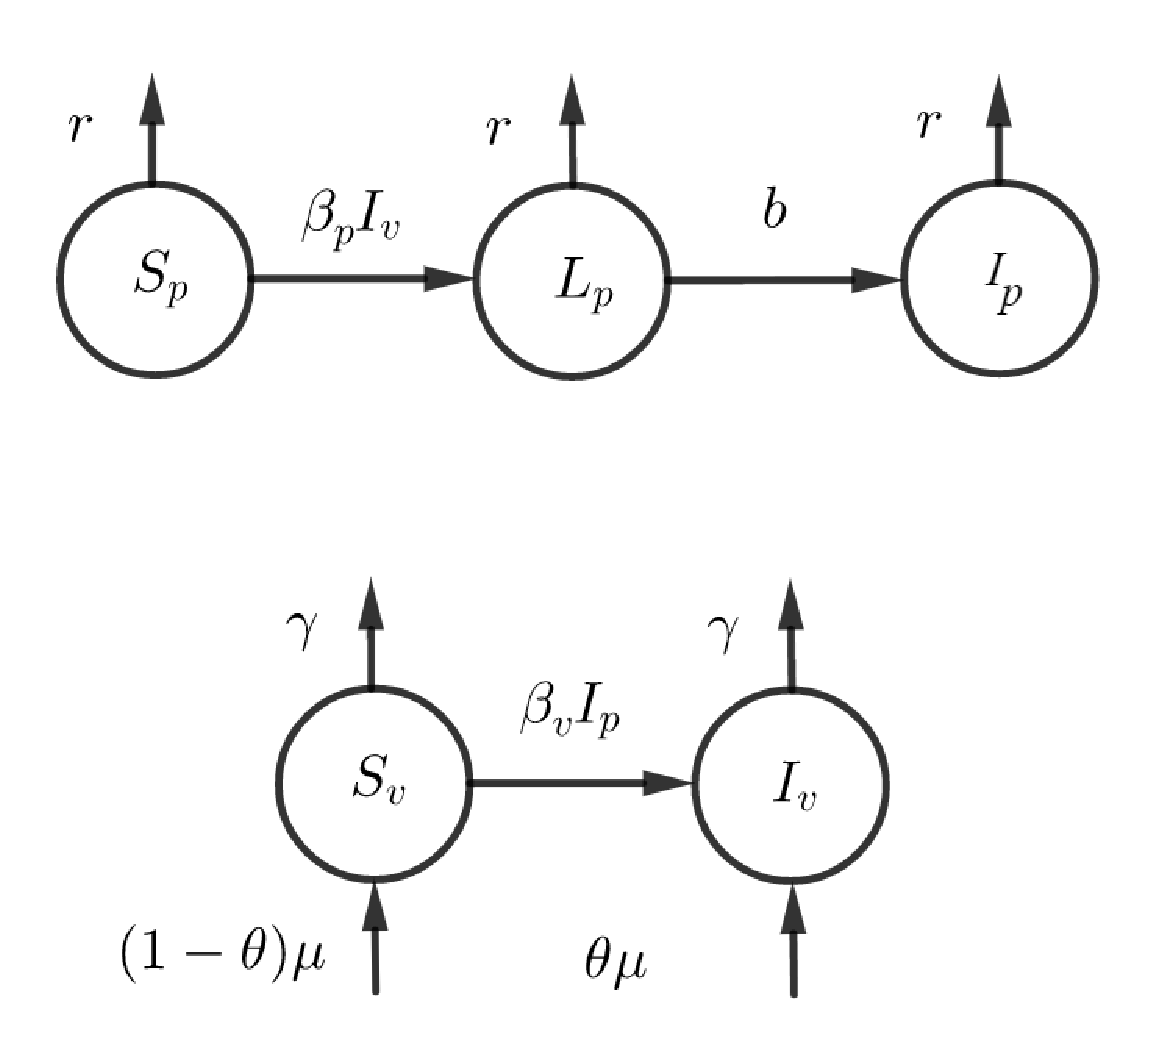
\includegraphics[scale= 0.3]{Feathergraphics/plant_diagram.eps}
  \caption{Diagram of dynamic in plants and vectors.}
  %\label{fig1}
\end{figure}
\end{frame}

\begin{frame}	
	Consider the following ordinary differential equations:
		\begin{eqnarray}
            \frac{dS_p}{dt} &=&-\beta_p S_p I_v +r (L_p +  I_p),\nonumber\\
            \frac{dL_p}{dt} &=& \beta_p S_p I_v -b L_p -r L_p,\nonumber\\
            \frac{dI_p}{dt} &=& b L_p - r I_p,\\
            \frac{dS_v}{dt} &=&-\beta_v S_v I_p - \gamma S_v -(1-\theta)\mu,\nonumber\\
            \frac{dI_v}{dt} &=&  \beta_v S_v I_p -\gamma I_v -\theta\mu\nonumber.
		\end{eqnarray}					
			%$$S_p(0) = S_p_0, L_p(0) = L_p_0, I_p(0) = I_p_0, S_v(0) = S_v_0, I_v(0) = I_v_0.$$				
\end{frame}

\begin{frame}
Computing the $R_0$ we have,

	$$R_0=\sqrt{\frac{\beta_v\mu b\beta_p}{r^2(r+b)\gamma}}$$


\begin{figure}
	\centering	
	\includegraphics[scale=0.3]{Feathergraphics/Tomato_simulation_1.eps}
	\includegraphics[scale= 0.3]{Feathergraphics/Tomato_simulation_2.eps}
	\caption{Evolution of infectious plants.}
	%\label{fig1}
\end{figure}	
\end{frame}
%-------------------------------------------------------
%-------------------------------------------------------

%-------------------------------------------------------
%-------------------------------------------------------
\section{Controlled Model}
\subsection{Plant model}
\begin{frame}{Plant Model with control}{Tomato Leaf Curl Virus Disease Using an Epidemiological Model}
The controlled system is the following:

    \begin{equation}
        \begin{aligned}
            \frac{dS_p}{dt} &=
                -\beta_p S_p I_v +(r +u_1)L_p + (r + u_2) I_p,
            \\
            \frac{dL_p}{dt} &=
                \beta_p S_p I_v -b L_p -(r + u_1)L_p,
            \\
            \frac{dI_p}{dt} &=
                b L_p - (r + u_2) I_p,
            \\
            \frac{dS_v}{dt} &=
                -\beta_v S_v I_p - (\gamma+u_3) S_v -(1-\theta)\mu,
            \\
            \frac{dI_v}{dt} &=
                \beta_v S_v I_p -(\gamma+u_3) I_v -\theta\mu,				
        \end{aligned}
    \end{equation}
\end{frame}

\begin{frame}
	With the cost functional:
	\begin{equation}
	\int_{0}^T
	\left[
	A_1 I_p(t) + A_2 L_p(t) + A_3 I_v(t)
	+ c_1 u_1(t)^2 + c_2 u_2(t)^2 + c_3 u_3(t)^2
	\right] dt,
	\end{equation}
		
\end{frame}

\begin{frame}
\begin{figure}
\frametitle{Case with one controls}
	\centering	
	\includegraphics[scale=0.5]{Feathergraphics/figure_1_tomato_one_control.eps}
	\caption{Evolution of infectious plants with one control, $u_3(t)$: Fumigation.}
	%\label{fig1}
\end{figure}	
\end{frame}

\begin{frame}
\begin{figure}
\frametitle{Case with two controls}

	\centering	
	\includegraphics[scale=0.5]{Feathergraphics/two_control_simulation_2.eps}
	\caption{Evolution of infectious plants with two controls, $u_1(t)$: removed latent plants, $u_2(t)$: removed infected plants.}
	%\label{fig1}
\end{figure}	
\end{frame}

\begin{frame}
\begin{figure}
\frametitle{Case with three controls}
	\centering	
	\includegraphics[scale=0.5]{Feathergraphics/three_controls_simulation_1.eps}
	\caption{Evolution of infectious plants with three controls, $u_1(t)$: removed latent plants, $u_2(t)$: removed infected plants, $u_3(t)$: Fumigation.}
	%\label{fig1}
\end{figure}	
\end{frame}



%-------------------------------------------------------
%-------------------------------------------------------
     

%-------------------------------------------------------
%-------------------------------------------------------

\end{document}